\chapter{Resultados de los distintos modelos \gls{rnn}}
\label{appendix:resultadosRNN}

La línea verde en los gráficos de tensorboard indican la mejor combinación de hiperparámetos encontrada en cada caso

\section{Intervalo 0.2s}

\begin{figure}[H]
    \centering
    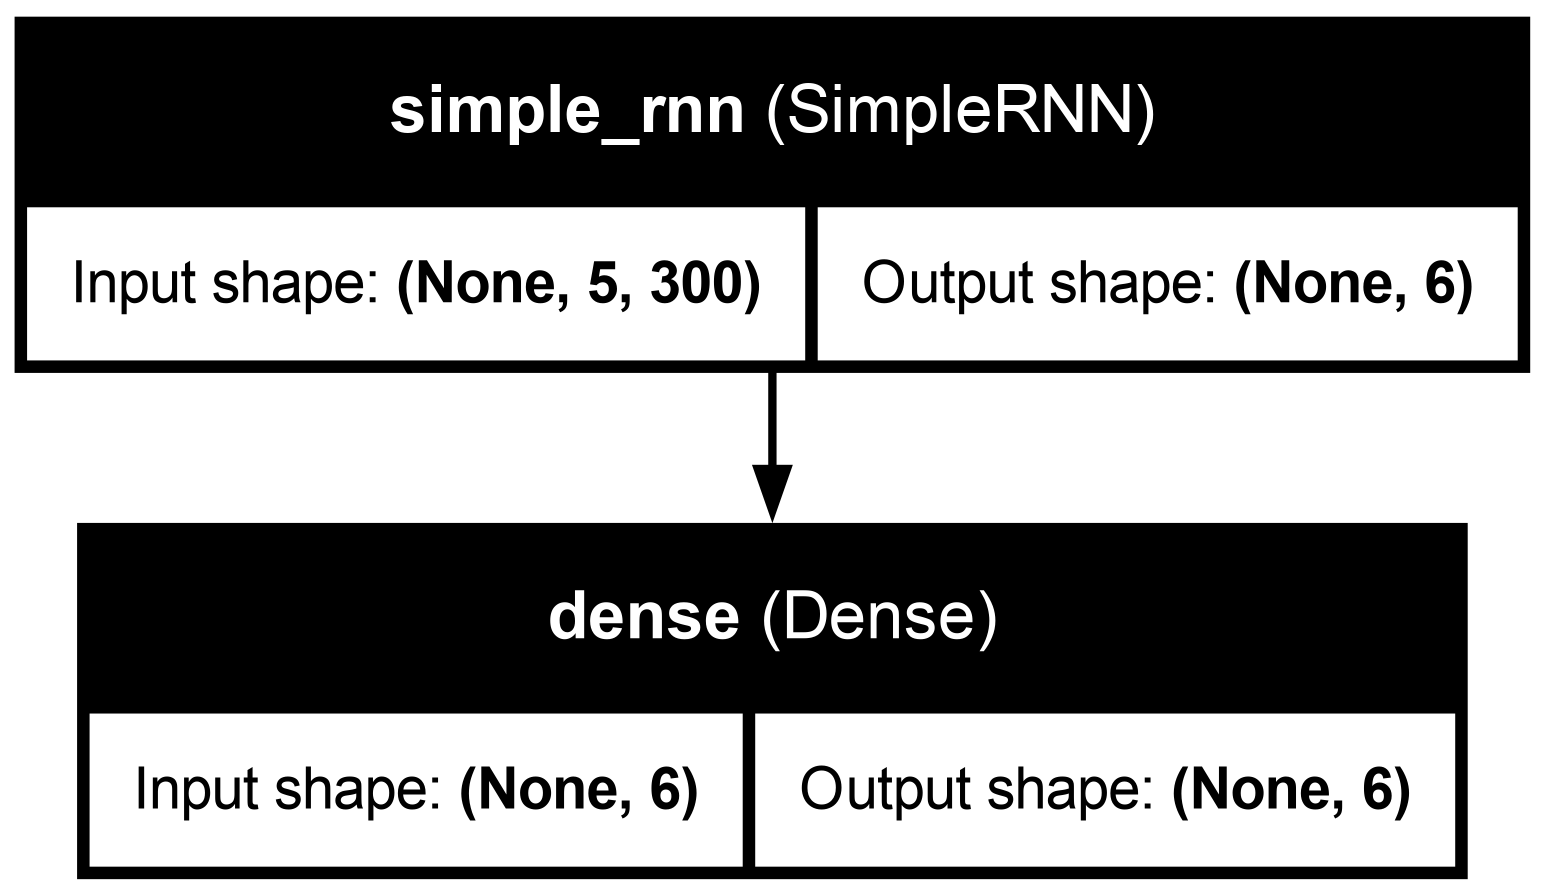
\includegraphics[width=0.3\textwidth]{Imagenes/Bitmap/best-rnn0.2.png}
    \caption{Esquema del modelo RNN con 0.2s de intervalo}
    \label{fig:rnn-0.2-final}
\end{figure}
\begin{figure}[H]
    \centering
    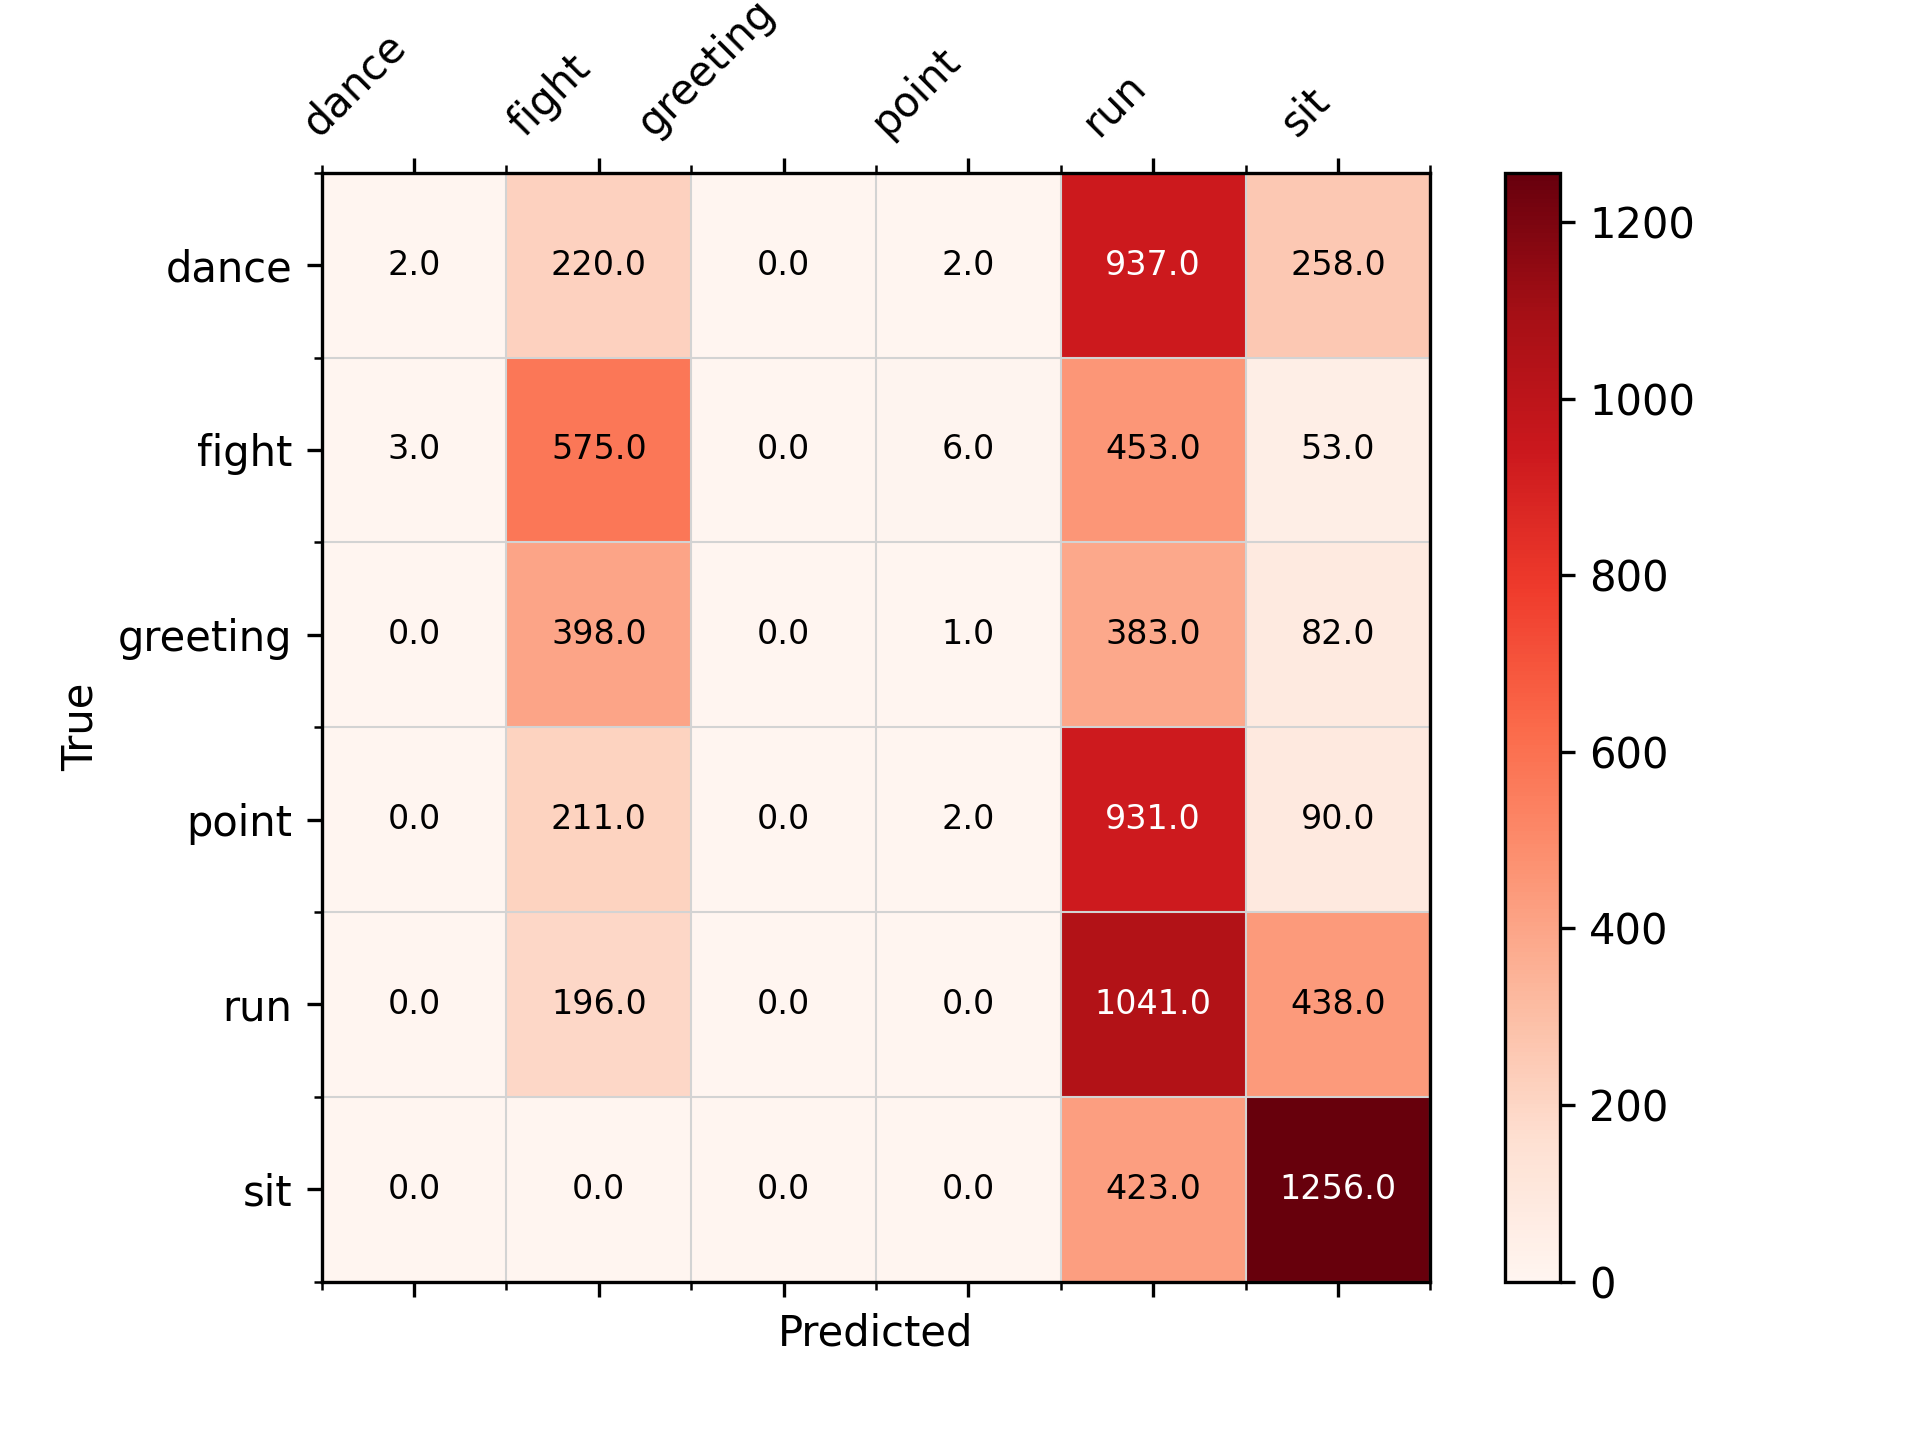
\includegraphics[width=0.6\textwidth]{Imagenes/Bitmap/CM_best-rnn0.2.png}
    \caption{Matriz de confusión del modelo RNN con 0.2s de intervalo}
    \label{fig:rnn-0.2-matriz}
\end{figure}
\begin{figure}[H]
    \centering
    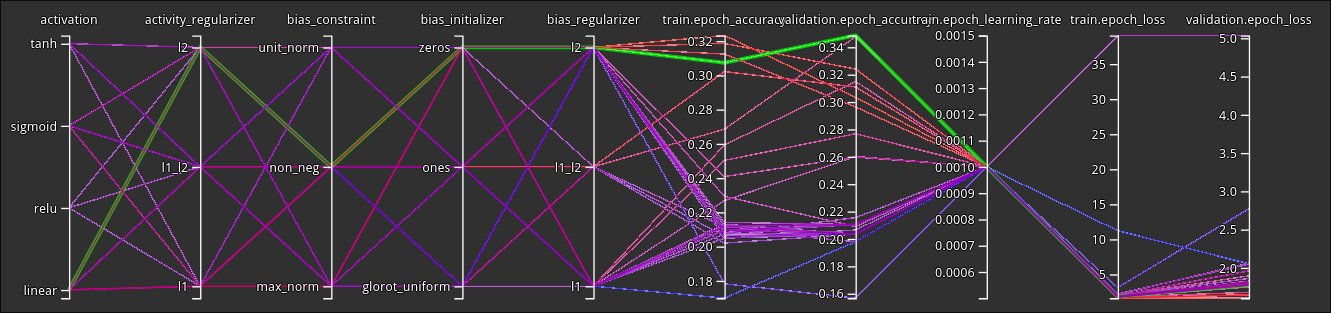
\includegraphics[width=0.8\textwidth]{Imagenes/Bitmap/tb-rnn-0.2.png}
    \caption{Gráfico de entrenamiento del modelo RNN con 0.2s de intervalo (mejor val\_accuracy = 0.3486)}
    \label{fig:rnn-0.2-grafico}
\end{figure}

\section{Intervalo 0.4s}

\begin{figure}[H]
    \centering
    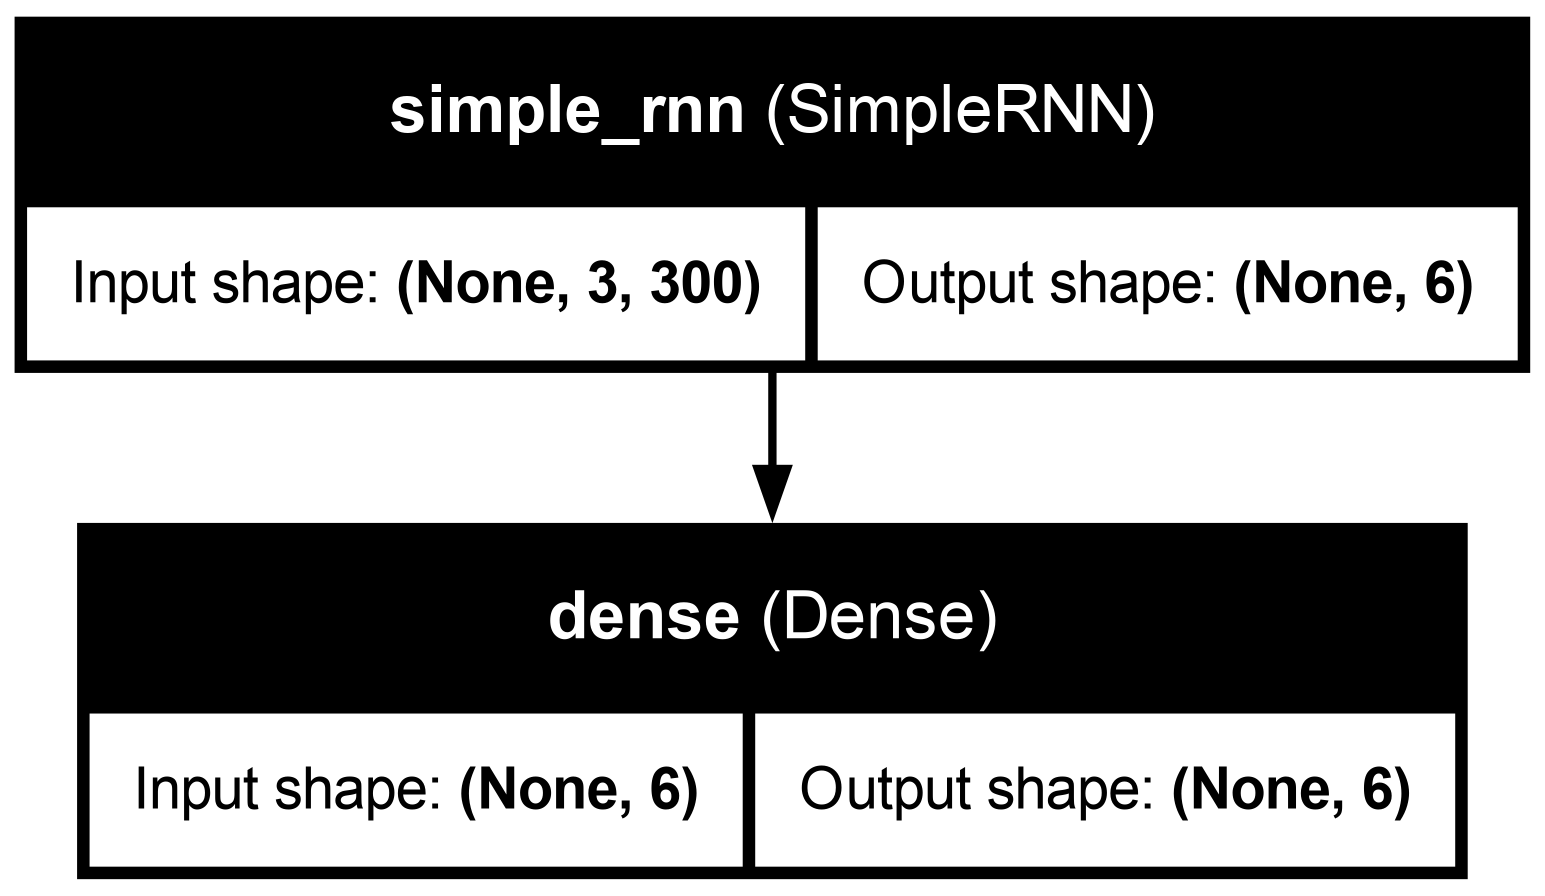
\includegraphics[width=0.3\textwidth]{Imagenes/Bitmap/best-rnn0.4.png}
    \caption{Esquema del modelo RNN con 0.4s de intervalo}
    \label{fig:rnn-0.4-final}
\end{figure}
\begin{figure}[H]
    \centering
    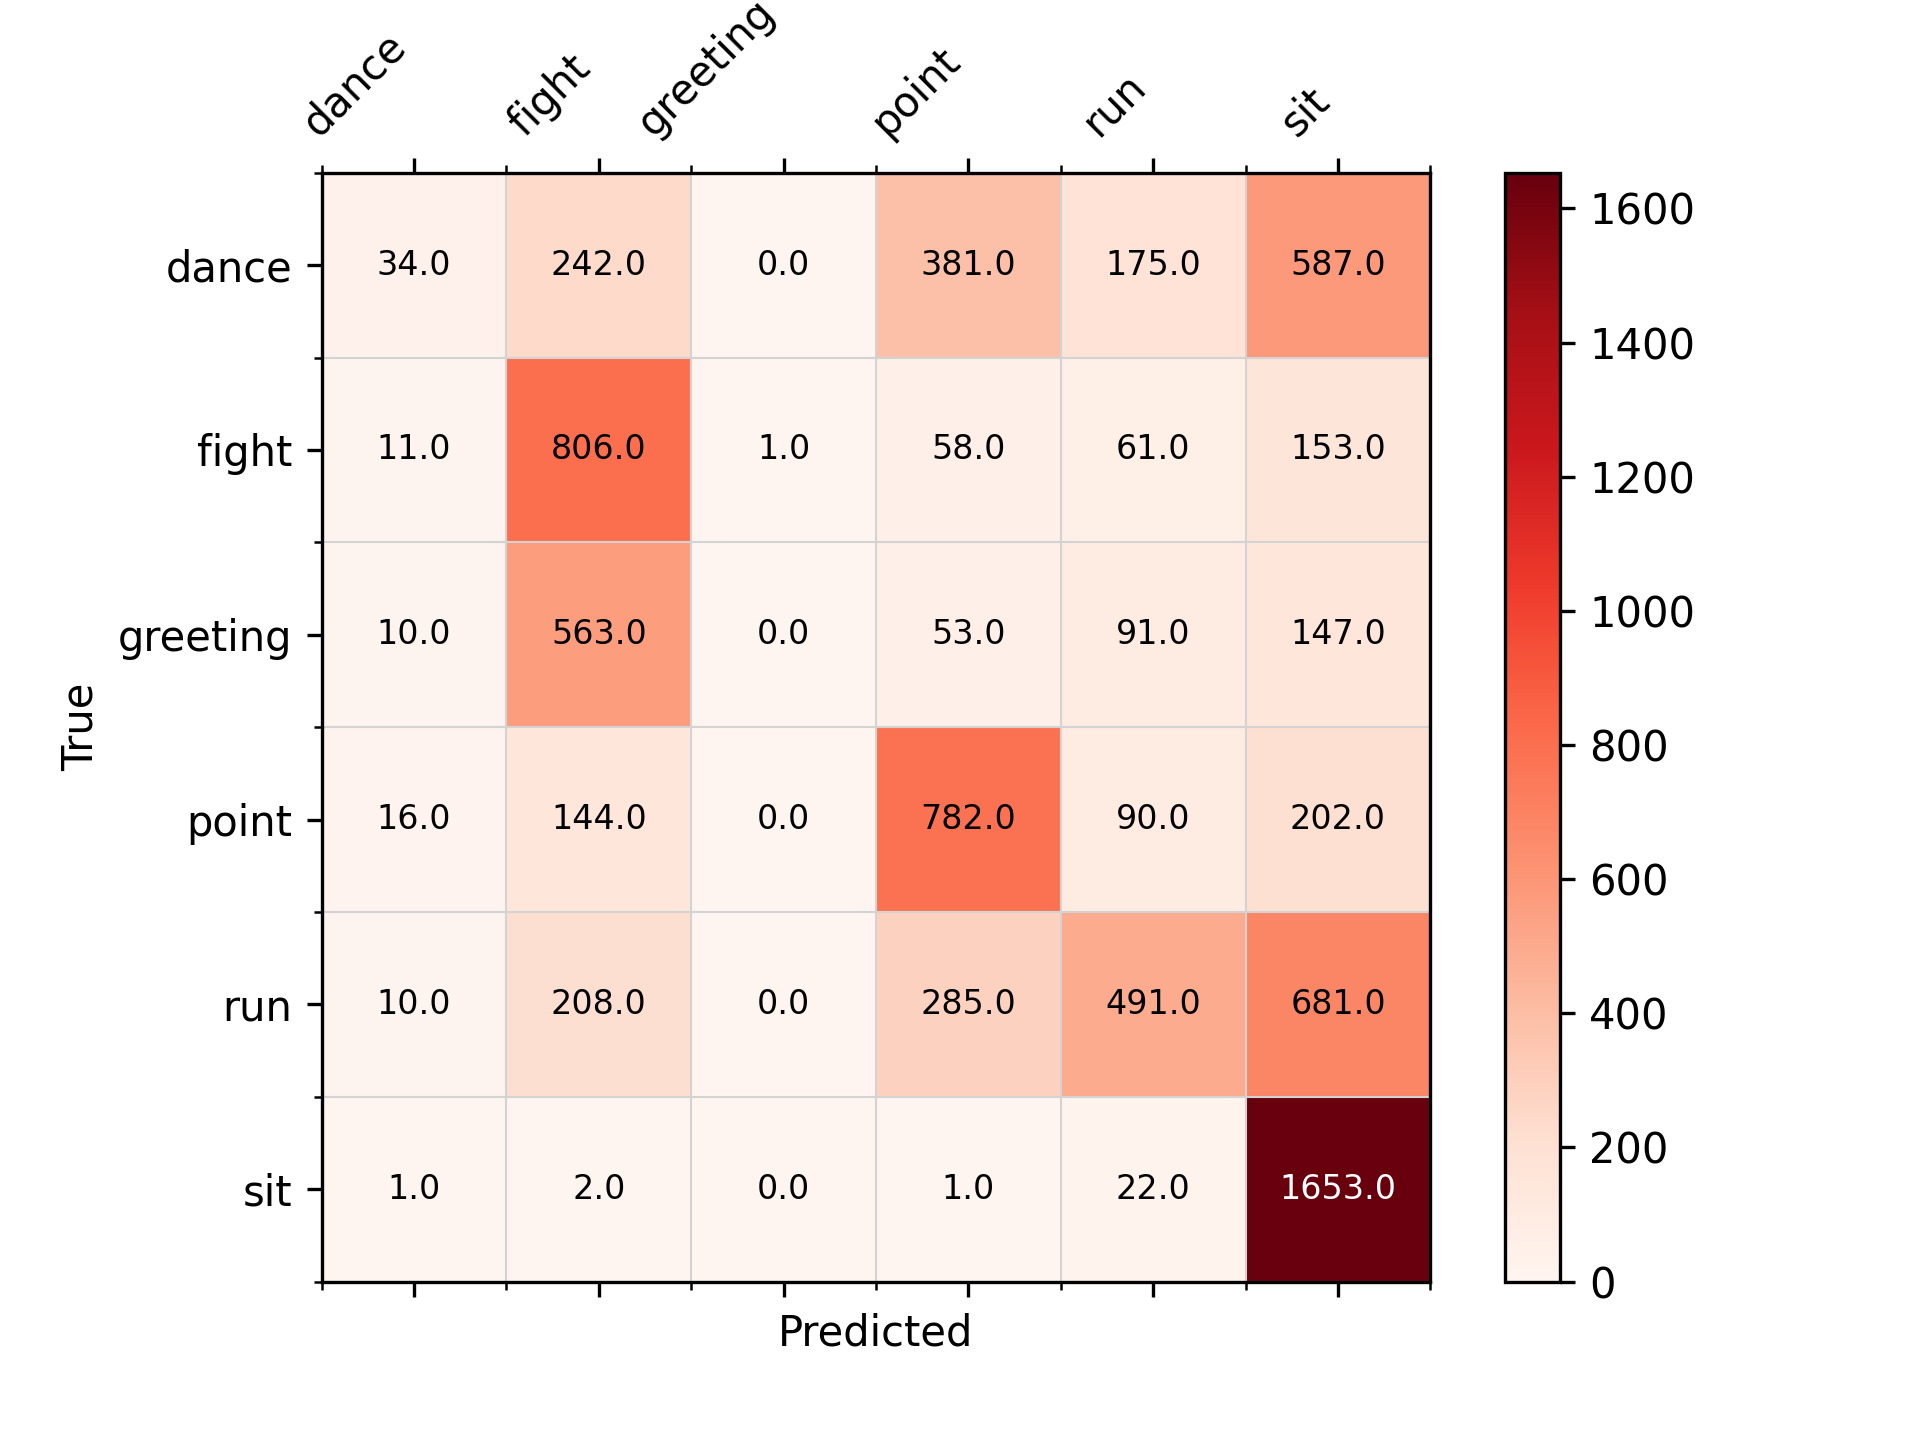
\includegraphics[width=0.6\textwidth]{Imagenes/Bitmap/CM_best-rnn0.4.png}
    \caption{Matriz de confusión del modelo RNN con 0.4s de intervalo}
    \label{fig:rnn-0.4-matriz}
\end{figure}

\begin{figure}[H]
    \centering
    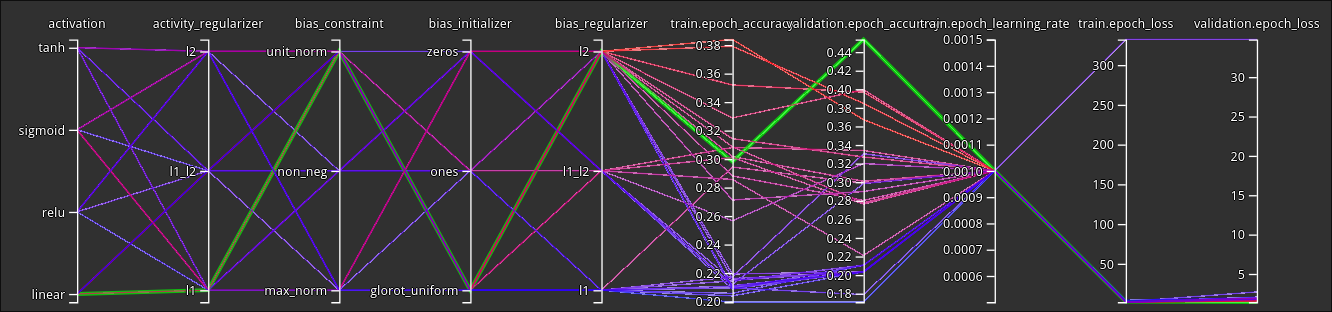
\includegraphics[width=0.8\textwidth]{Imagenes/Bitmap/tb-rnn-0.4.png}
    \caption{Gráfico de entrenamiento del modelo RNN con 0.4s de intervalo (mejor val\_accuracy = 0.4535)}
    \label{fig:rnn-0.4-grafico}
\end{figure}

\section{Intervalo 0.6s}

\begin{figure}[H]
    \centering
    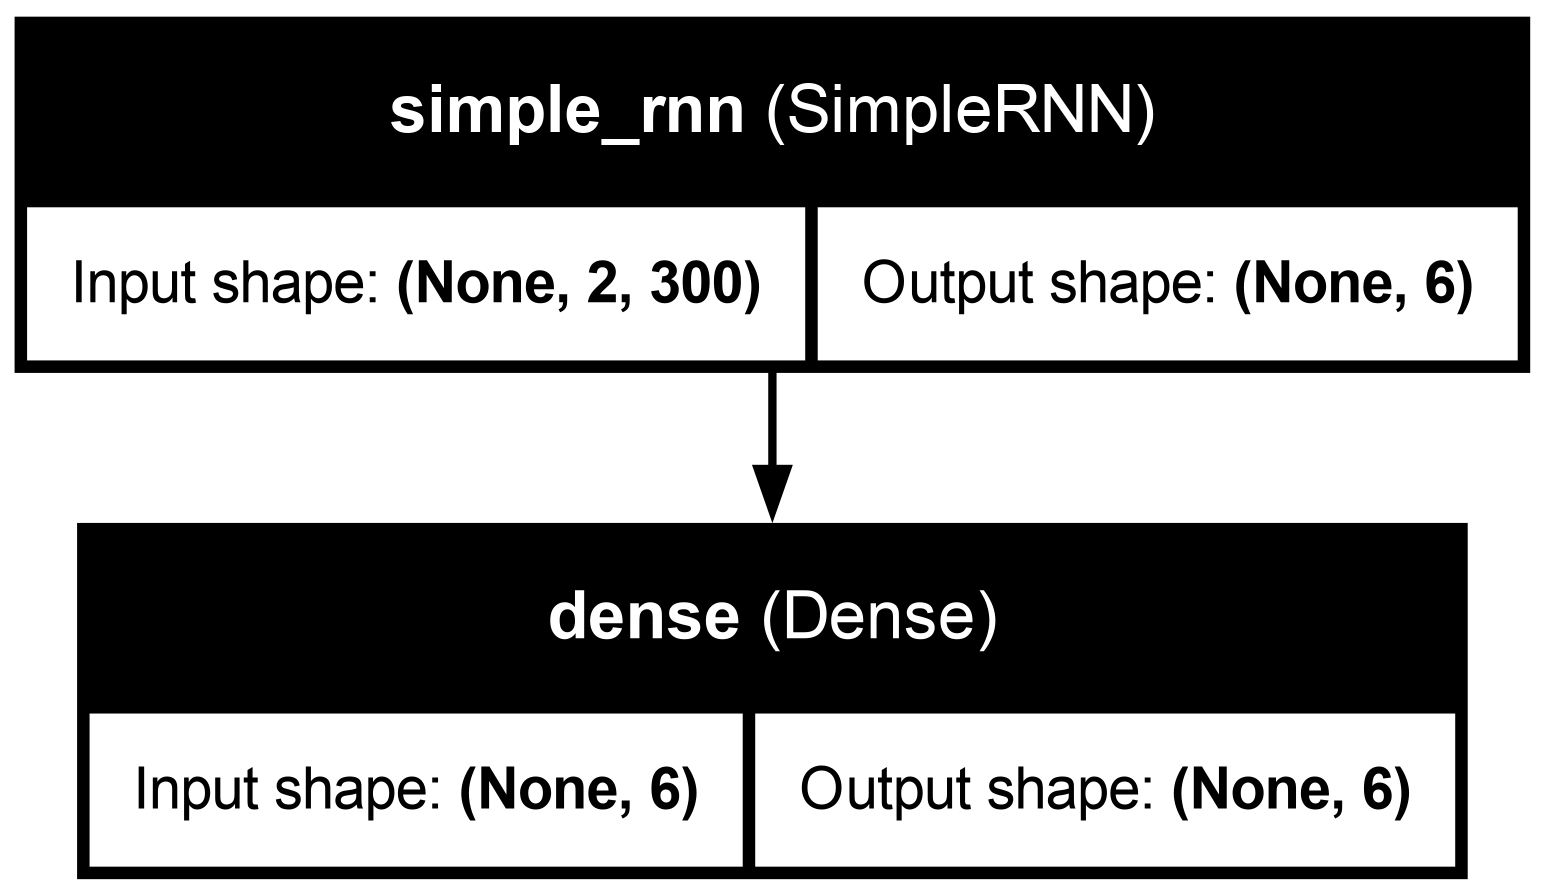
\includegraphics[width=0.3\textwidth]{Imagenes/Bitmap/best-rnn0.6.png}
    \caption{Esquema del modelo RNN con 0.6s de intervalo}
    \label{fig:rnn-0.6-final}
\end{figure}

\begin{figure}[H]
    \centering
    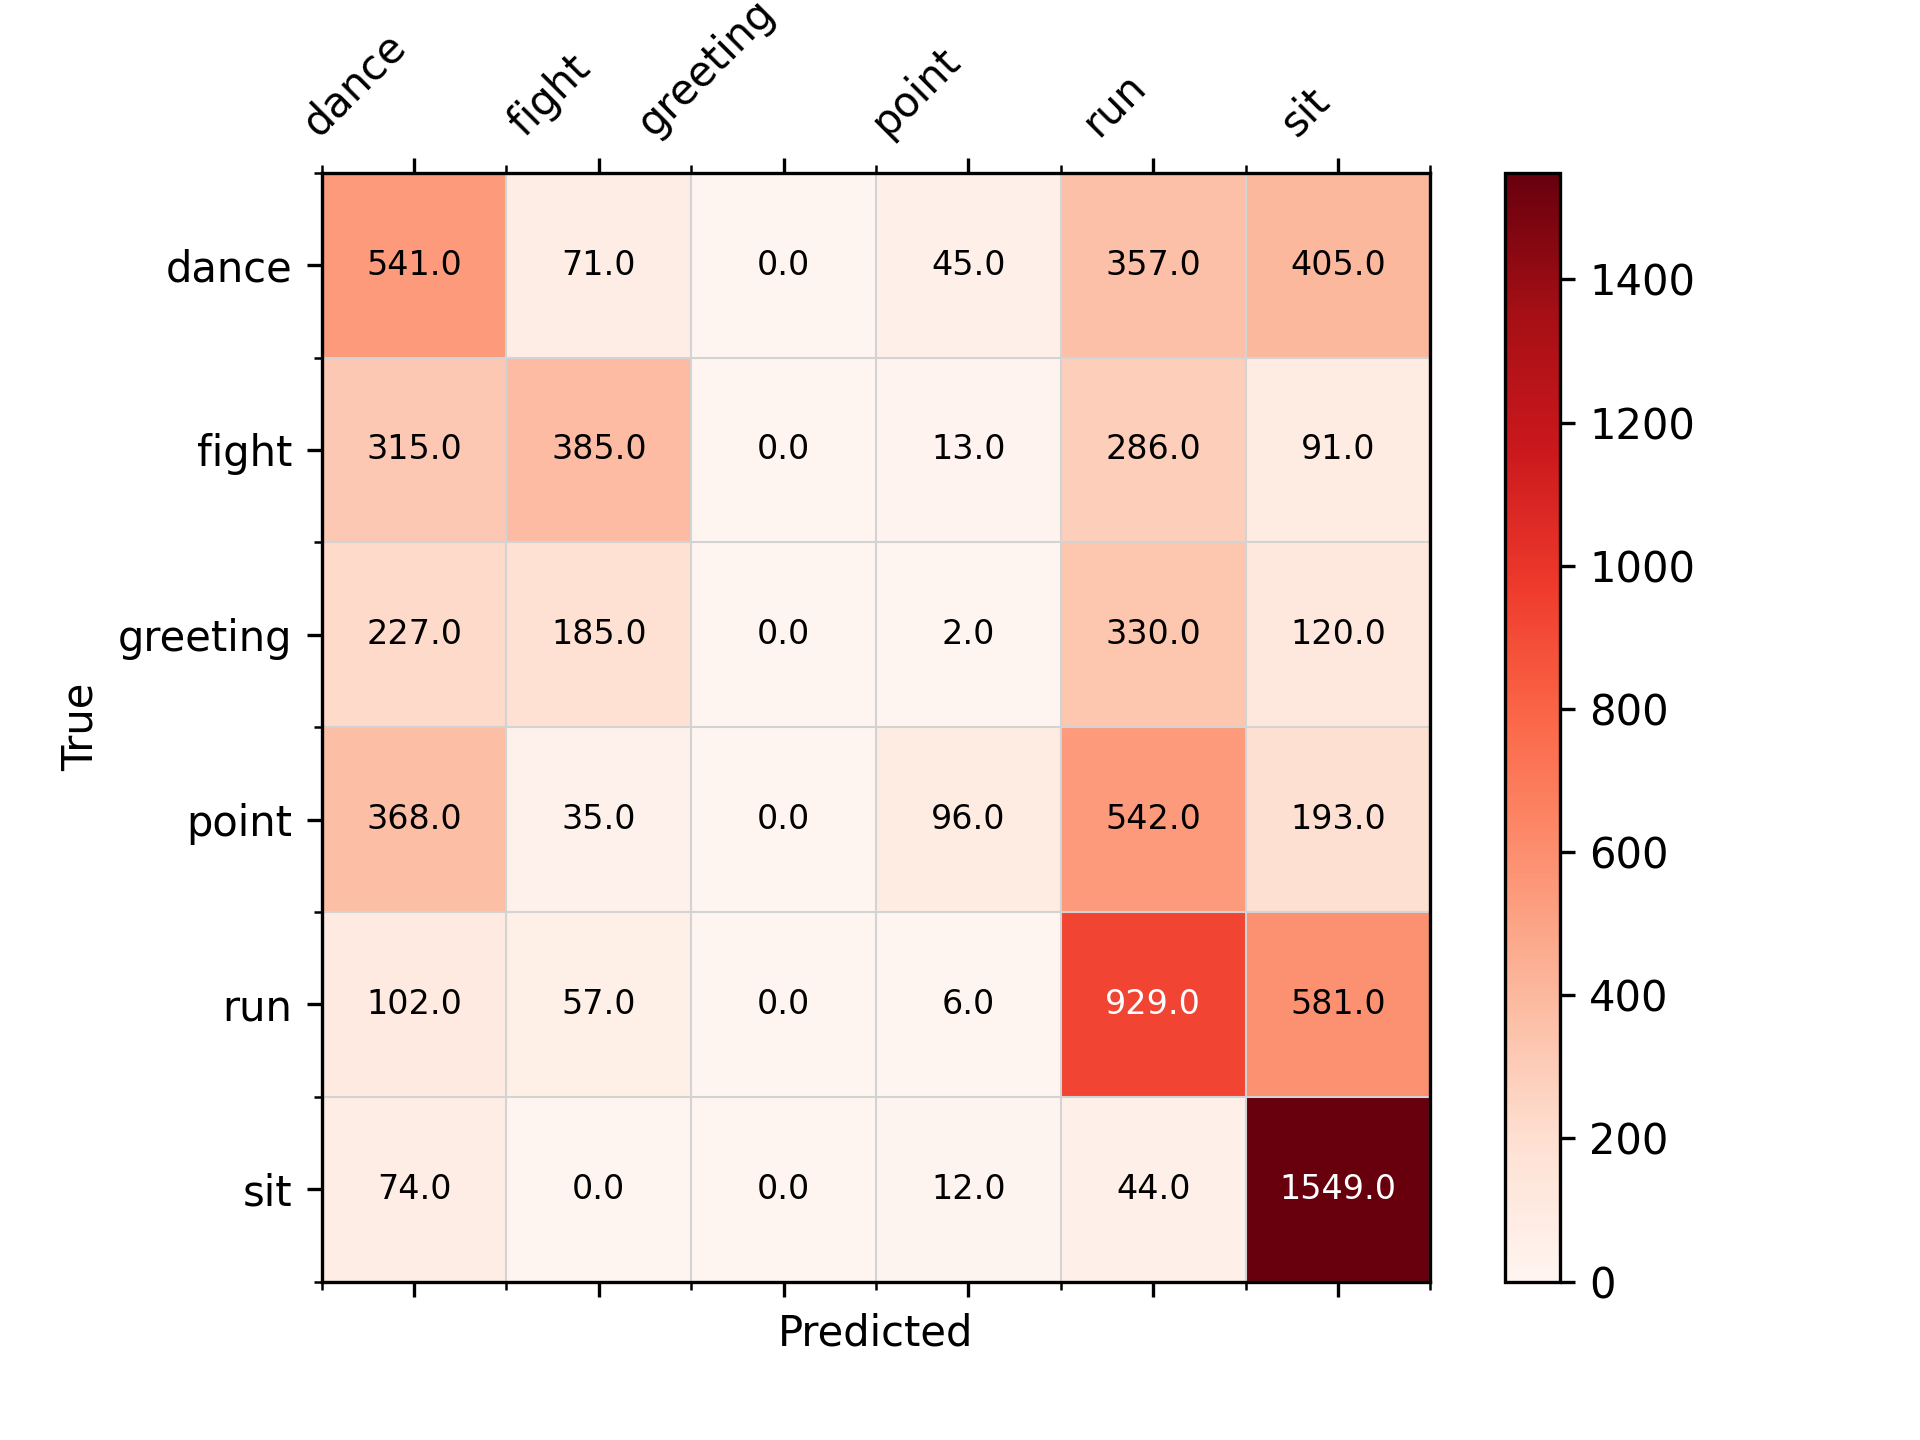
\includegraphics[width=0.6\textwidth]{Imagenes/Bitmap/CM_best-rnn0.6.png}
    \caption{Matriz de confusión del modelo RNN con 0.6s de intervalo}
    \label{fig:rnn-0.6-matriz}
\end{figure}

\begin{figure}[H]
    \centering
    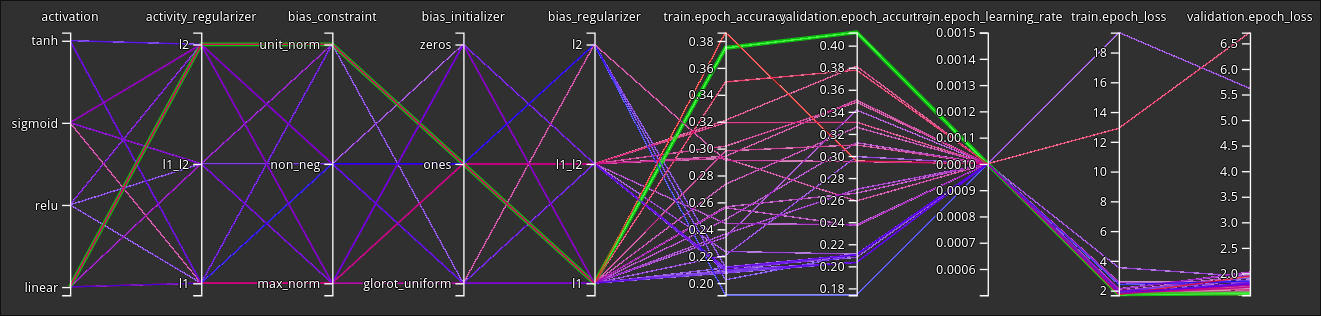
\includegraphics[width=0.8\textwidth]{Imagenes/Bitmap/tb-rnn-0.6.png}
    \caption{Gráfico de entrenamiento del modelo RNN con 0.6s de intervalo (mejor val\_accuracy = 0.41185)}
    \label{fig:rnn-0.6-grafico}
\end{figure}

\section{Intervalo 0.8s}

\begin{figure}[H]
    \centering
    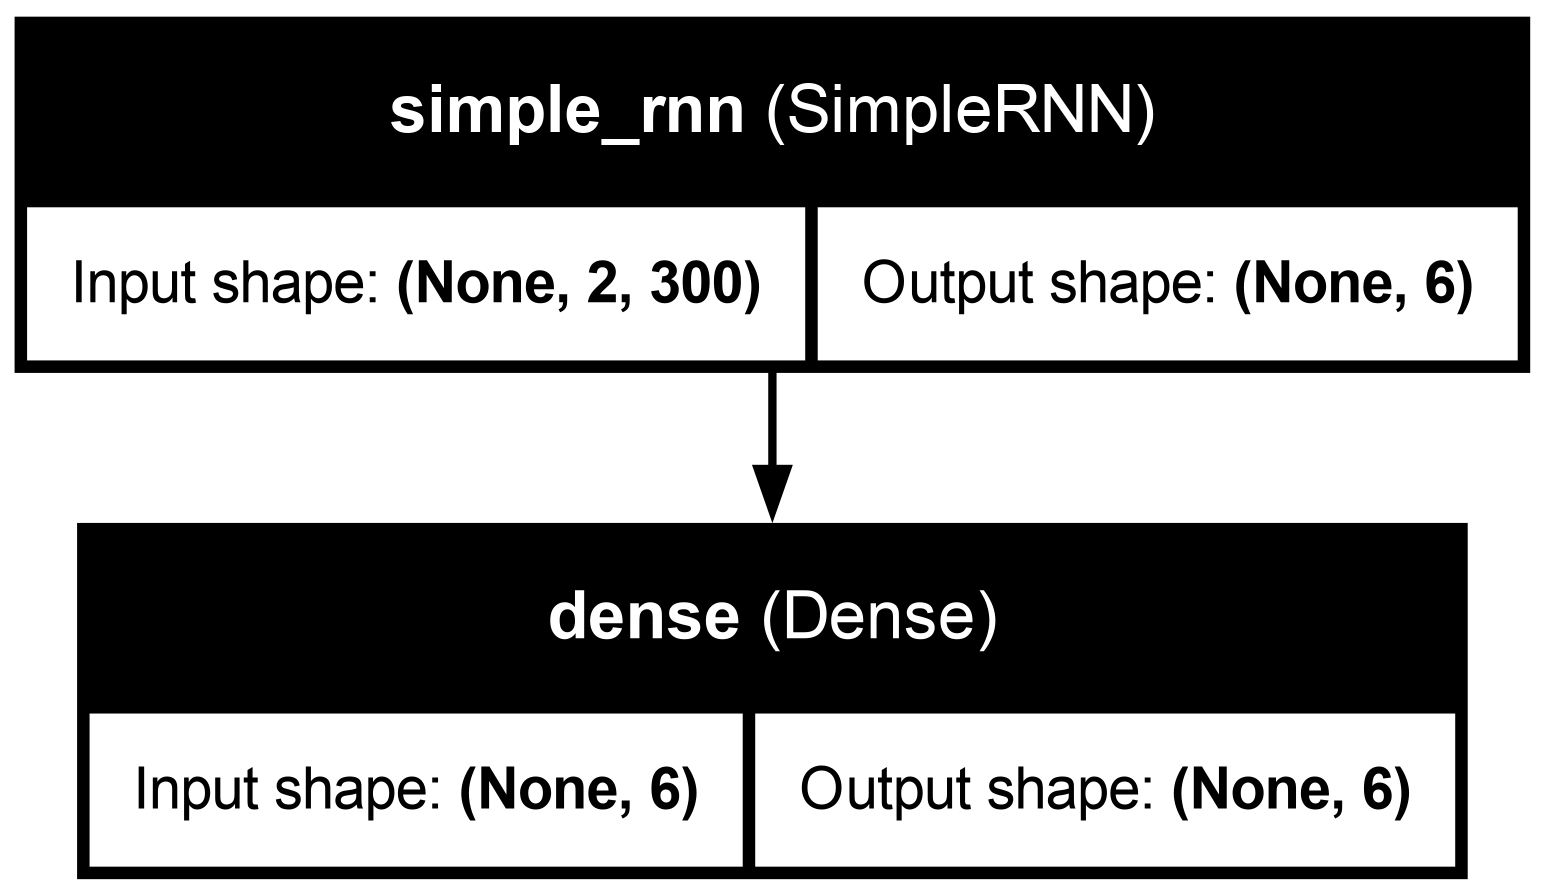
\includegraphics[width=0.3\textwidth]{Imagenes/Bitmap/best-rnn0.8.png}
    \caption{Esquema del modelo RNN con 0.8s de intervalo}
    \label{fig:rnn-0.8-final}
\end{figure}

\begin{figure}[H]
    \centering
    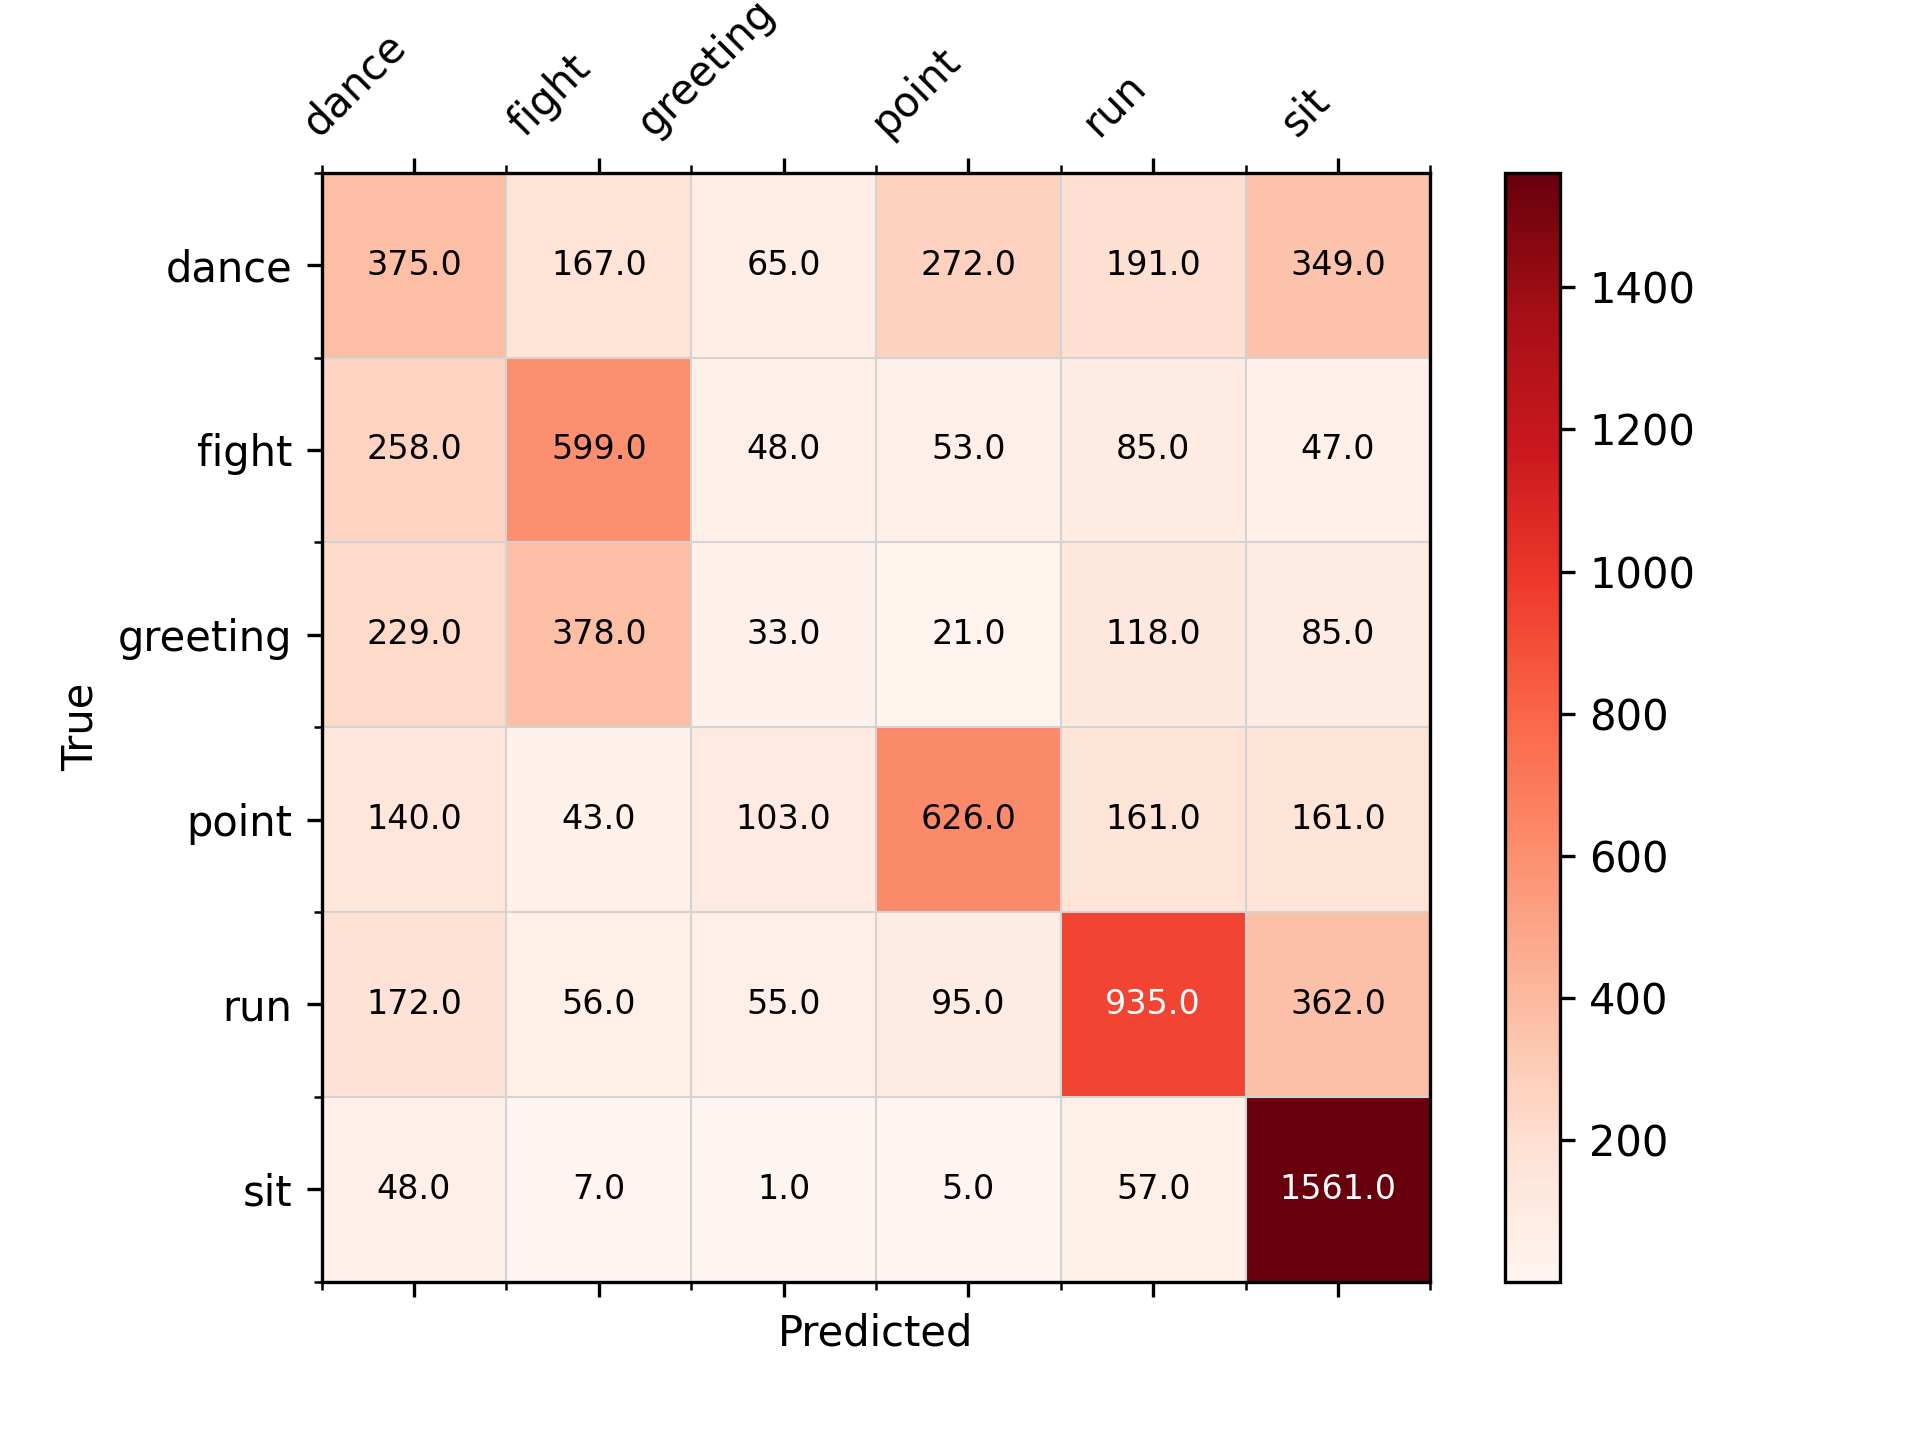
\includegraphics[width=0.6\textwidth]{Imagenes/Bitmap/CM_best-rnn0.8.png}
    \caption{Matriz de confusión del modelo RNN con 0.8s de intervalo}
    \label{fig:rnn-0.8-matriz}
\end{figure}

\begin{figure}[H]
    \centering
    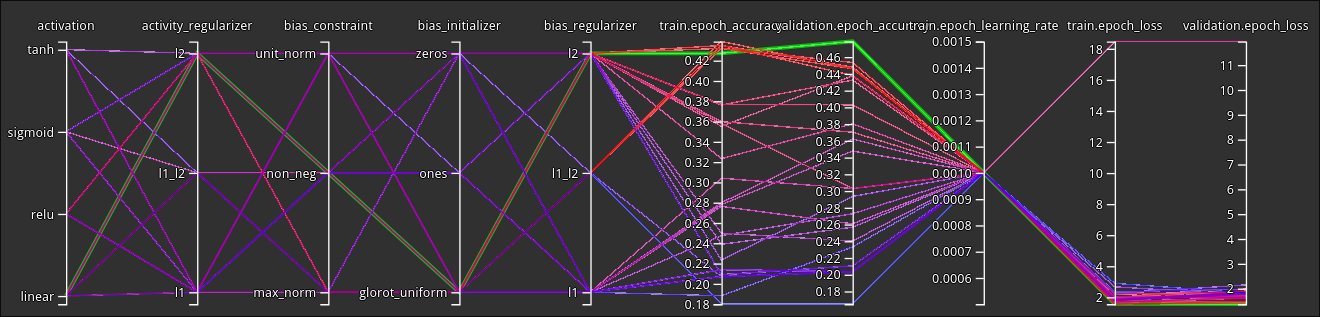
\includegraphics[width=0.8\textwidth]{Imagenes/Bitmap/tb-rnn-0.8.png}
    \caption{Gráfico de entrenamiento del modelo RNN con 0.8s de intervalo (mejor val\_accuracy = 0.47865)}
    \label{fig:rnn-0.8-grafico}
\end{figure}

\section{Intervalo 1.0s}

\begin{figure}[H]
    \centering
    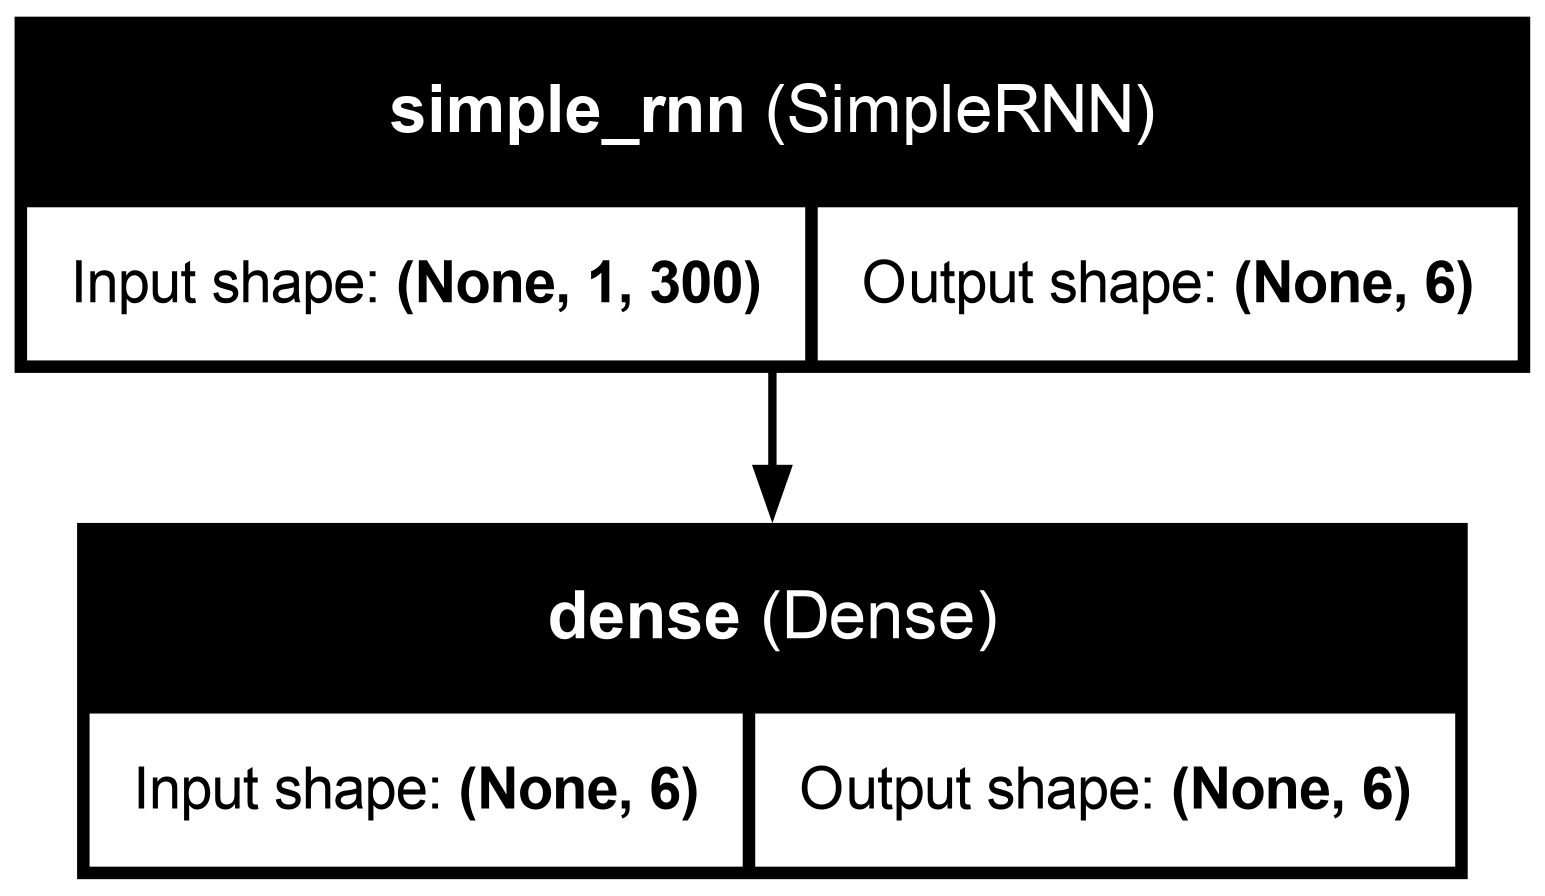
\includegraphics[width=0.3\textwidth]{Imagenes/Bitmap/best-rnn1.0.png}
    \caption{Esquema del modelo RNN con 1.0s de intervalo}
    \label{fig:rnn-1.0-final}
\end{figure}

\begin{figure}[H]
    \centering
    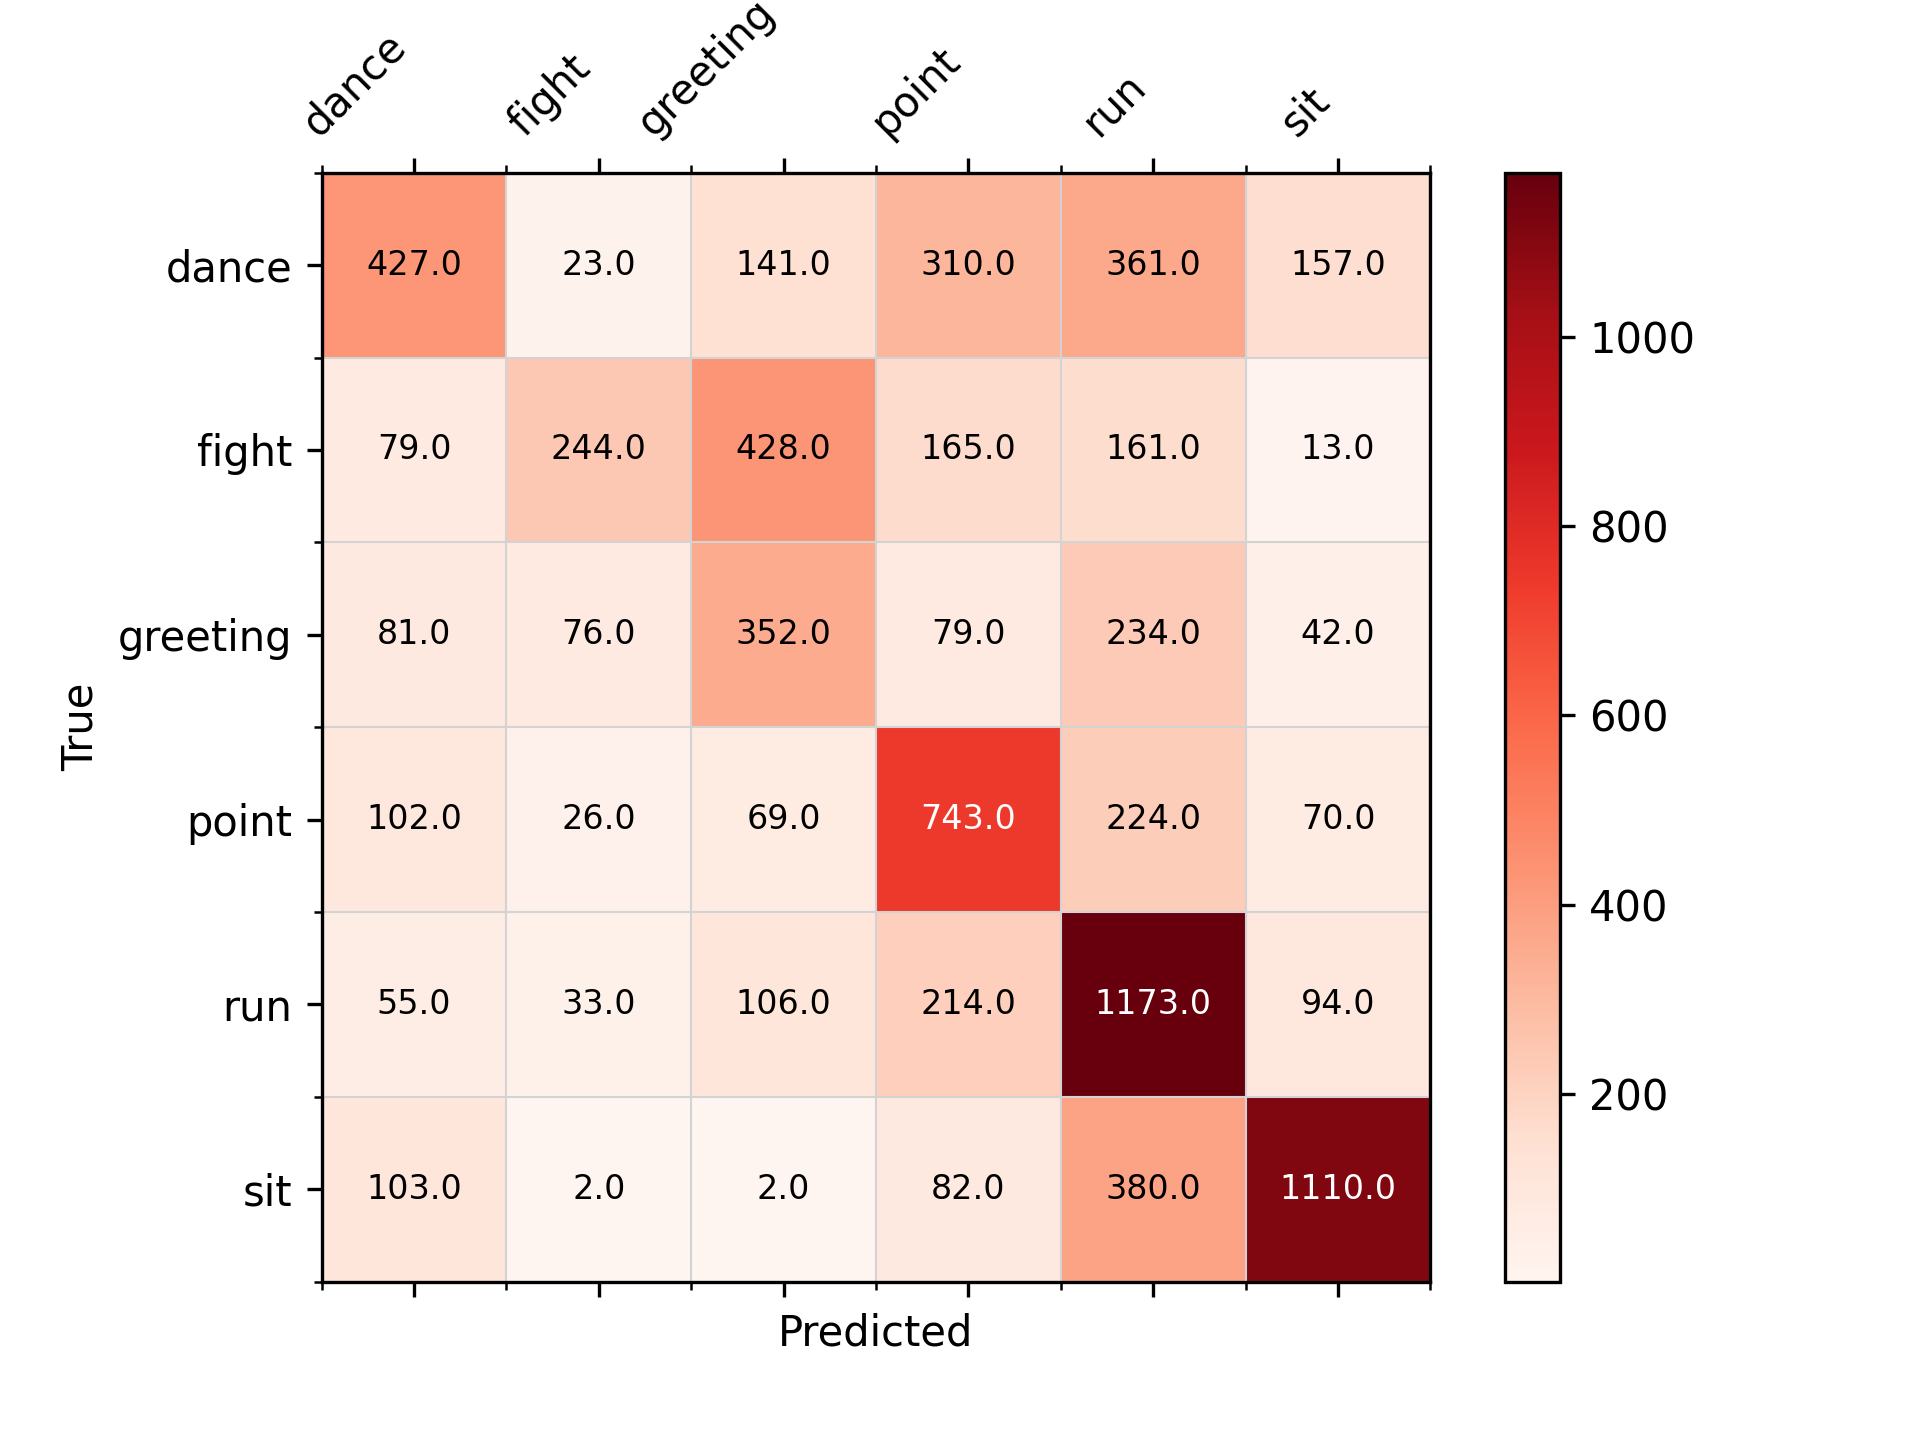
\includegraphics[width=0.6\textwidth]{Imagenes/Bitmap/CM_best-rnn1.0.png}
    \caption{Matriz de confusión del modelo RNN con 1.0s de intervalo}
    \label{fig:rnn-1.0-matriz}
\end{figure}

\begin{figure}[H]
    \centering
    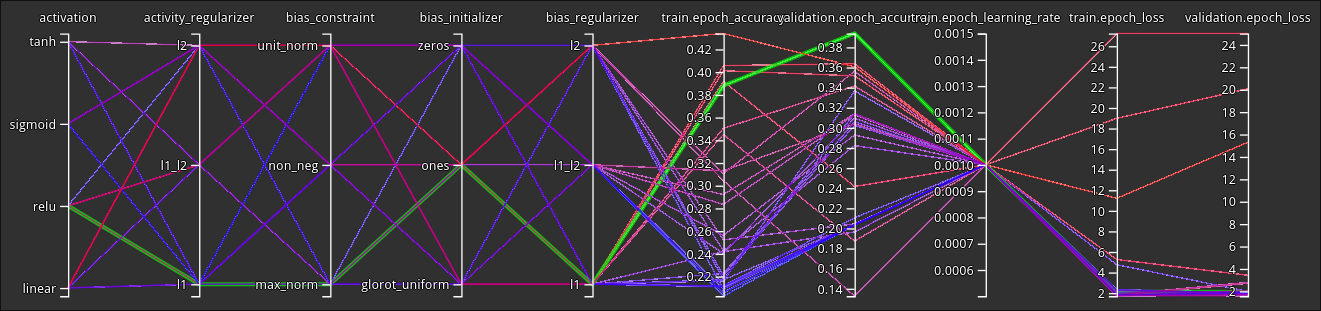
\includegraphics[width=0.8\textwidth]{Imagenes/Bitmap/tb-rnn-1.0.png}
    \caption{Gráfico de entrenamiento del modelo RNN con 1.0s de intervalo (mejor val\_accuracy = 0.39377)}
    \label{fig:rnn-1.0-grafico}
\end{figure}